\chapter{THEORETICAL AND CONCEPTUAL FRAMEWORKS}\label{ch:tf-cf}
The theories from the literatures reviewed in the preceding chapter will be discussed in this chapter. In addition to this, the solutions will be presented at a high level through the conceptual framework, where the details will be discussed in the methodologies.
\section{Theoretical Framework}
As established in Chapter~\ref{ch:rrl}, statistical analyses of the morphological characteristics of the Qur'\=an's corpus \shortcite{dukes-habash-2010-morphological} have predominantly focused on comparative studies with other corpora. However, no research has examined the positional statistics of morphological features for specific entities such as God's names or prophets' names. Investigating these patterns will help us in understanding the Qur'\=an's structure by studying how these entities are distributed throughout the text and their relationship to the \arb[trans]{'asbAb 'alnuzUl} \arb{'asbAb 'alnuzUl} (occasions or circumstances of revelation). Additionally, examining unique morphological features in early extant manuscripts represents an unexplored avenue that this study will address.

The work of \shortciteA{siddiqui2013}, discussed in Chapter~\ref{ch:rrl}, employed Latent Dirichlet Allocation (LDA) on 24 \arb[trans]{sUwar} \arb{sUwar} using Term Frequency-Inverse Document Frequency (TF-IDF) as word embeddings. While this approach proved effective, recent advances in Large Language Models (LLMs) have produced superior word embeddings, particularly the Bidirectional Encoder Representations from Transformers (BERT) models \shortcite{devlin2018bert}. BERT models, as detailed in Section~\ref{sec:bert}, surpass TF-IDF through their lower-dimensional embeddings that are independent of vocabulary size. Semantically, BERT demonstrates superior performance through its \textit{attention mechanism}\footnote{See Section~\ref{sec:attention-mechanism}}, which incorporates contextual information from surrounding words. Although LDA and BERTopic \cite{grootendorst2022bertopic} represent effective statistical methodologies for topic modeling, this study employs Generative Pre-trained Transformer (GPT) models for their superior summarization capabilities. Given that the Qur'\=an constitutes one of the world's most widely studied texts, commercial GPT models such as ChatGPT and Claude are well-acquainted with its content, having been trained on comprehensive textual datasets that include such prominent works.

Regarding \textit{rhythmic analyses} of Qur'\=anic texts, no prior research has approached this domain from a statistical perspective. This study provides the first mathematical formulation for such analyses and demonstrates their application to statistical methodologies. The analytical framework includes cluster analysis to identify groupings of \arb[trans]{sUwar} \arb{sUwar} based on rhythmic statistics, as well as examination of transition probabilities governing changes in rhythmic syllables throughout the Qur'\=an. Additional methodologies encompass descriptive statistics to characterize the rhythmic signatures of \arb[trans]{sUwar} \arb{sUwar} according to their revelation context, specifically whether they are \arb[trans]{makkiyyaT} \arb{makkiyyaT} (Meccan) or \arb[trans]{madaniyyaT} \arb{madaniyyaT} (Medinan).

Concerning the \textit{theory of concentrism}, this study faces a similar pioneering situation as with rhythmic analysis, being the first to provide a rigorous mathematical formulation of the theory. A significant criticism of \shortciteA{farrin2014structure}'s work, as noted by \shortciteA{sinai2017review}, concerns the arbitrary nature of structural boundary selection between concentric pattern groups, which lacks clear methodological guidelines. To address this limitation, this study proposes an optimization algorithm designed to identify optimal structural boundaries for concentric pattern groups. The algorithm employs Genetic Algorithm optimization, which will be formulated and presented as a key contribution of this thesis.

\section{Conceptual Framework}
Having discussed the theoretical framework of this paper, the proposed solution to the research questions postulated in Section \ref{sec:research_questions} will be discussed in this section at a conceptual level. Technically, the objectives of this paper can be divided into four: \textit{positional statistics}, \textit{morphological feature analyses}, \textit{thematic analyses}, \textit{rhythmic analyses}, \textit{concentric analyses}, and \textit{extant manuscript investigation}. Thus, the conceptual framework will be discussed according to these general objectives.
\subsection{Positional Statistics}
To study the positional statistics, like the \arb[trans]{'ayaT} \arb{'ayaT} counts, the \arb[trans]{suwar} \arb{suwar} counts, including the counts of its words and characters, the main tools that will be used are Julia libraries called QuranTree.jl \cite{asaad2021qurantree} and Yunir.jl \shortcite{al_ahmadgaid_b_asaad_yunir}. Using these tools, the distributions are then computed using other Julia libraries like Makie.jl for visualization, and Statistics.jl for computing the needed summary statistics.
\subsection{Morphological Feature Analyses}
As for the morphological analysis of the root word \arb[trans]{Alh} \arb[novoc]{Alh}, the goal is to simply find all of the locations of its morphologies (positional statistics), and then study those that are very unique by looking into the extant manuscripts to see if such morphologies are already present in the early extant manuscripts. 
\subsection{Rhythmic Analyses}
Since the rhythmic analyses at textual level have not been analyzed, this paper will explore different ways to studying the rhythm of the Qur'\=an, starting with syllabification of each \arb[trans]{'ayaT} \arb{'ayaT}, which basically splits each word of the \arb[trans]{'ayaT} \arb{'ayaT} into its syllables, and then assigning a prolongation score to it, which will then be analyzed with visualization, summary statistics, and transition probabilities.
\subsection{Concentric Analyses}
As for the concentric analysis, the paper will start with the mathematical formulation, this is the first paper to do so to the best knowledge of the author. The main algorithm that will be used is the Genetic Algorithm (GA).
\begin{figure}
    \label{fig:conceptual-framework}
    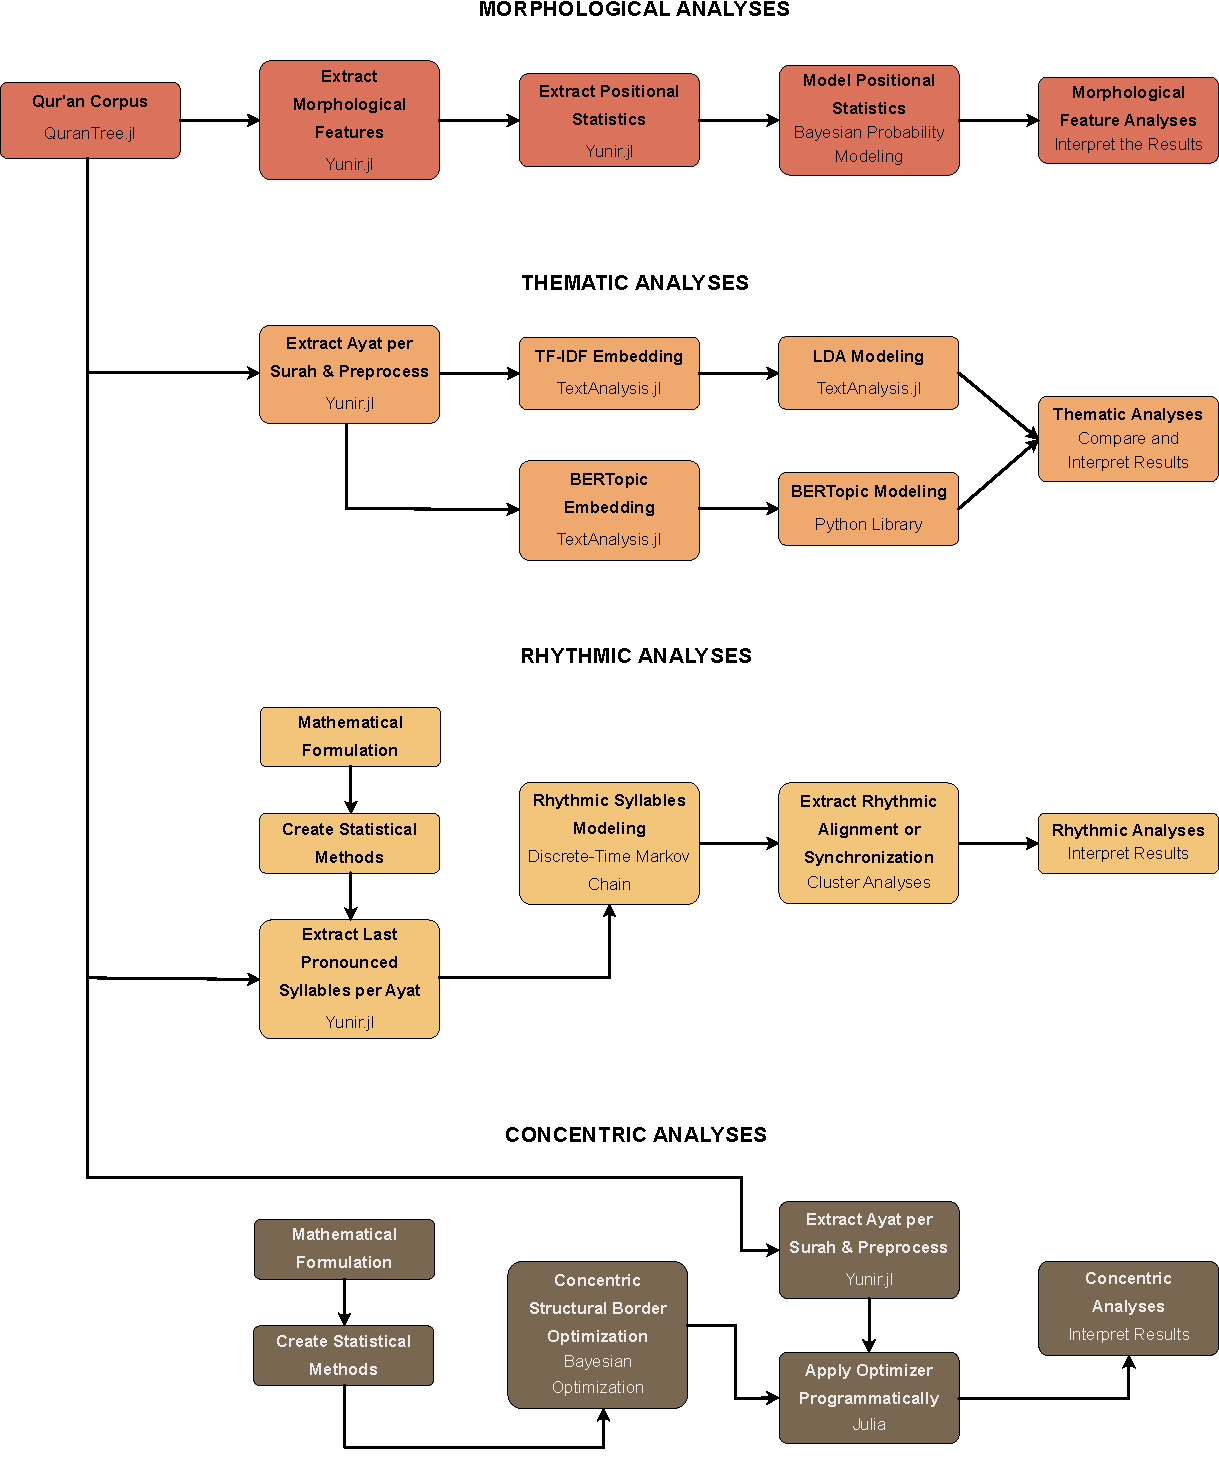
\includegraphics[width=\textwidth]{img/conceptual_framework.pdf}
    \vspace{2cm}
    \caption{Diagram of Conceptual Framework}
\end{figure}
\subsection{Thematic Analyses}
As mentioned in the theoretical framework, the topic modeling or thematic analyses can also be done with the BERTopic \shortcite{grootendorst2022bertopic}, but this study will use GPT \cite{radford2018improving} model. This is applied to the summarization of the result of the concentric analysis discussed in the preceding section.